\chapter{Rotational modulation in KIC\,2569073 an Ap star}

\section*{abstract}
    In this chapter we analyse KIC\,2569073\footnote[2]{Within the asteroseismology community there is a tradition of nicknaming stars with interesting light curves after pets. KIC\,2569073 is thus nicknamed Fluffy.}, an individual, non-targeted \Kepler superstamp star. It was initially considered to be a possible Cepheid variable star based on its photometric light curve. This would make it only the second known Cepheid in the nominal \Kepler field of view. We conclude however, that this is a non-oscillating Ap (noAp) star exhibiting rotational modulation, based upon multi-colour photometry and spectroscopic observations that eliminate the possibility of Cepheid classification.
    % \bigskip
\newpage
\section{Investigation of KIC\,2569073}

%We begin by providing a short introduction to Cepheid and A type stars that were the focus of this research and present additional details of the investigation prior to the paper itself.

During the initial SAP investigation of the \Kepler superstamps discussed in the previous chapter we discovered a particularly interesting light curve for KIC\,2569073. The light curve, extracted using a custom aperture derived for each quarter, showed an almost-sinusoidal variability reminiscent of classical Cepheid variable stars. 

Classical Cepheids are luminous giant and supergiant stars of spectral types F6-K2 \citep{rodgers_radius_1957} corresponding to stellar masses between 4\,\Msol~and 20\,\Msol~\citep{turner_progenitors_1996}. %The $\kappa$ mechanism acts within the helium ionisation zone of these stars to produce radial pulsations in these stars \citep{Eddington17}. These pulsations cause 
Cepheids show precise period variations in luminosity due to radial pulsations produced by the $\kappa$-mechanism acting in the helium ionisation zone \citep{eddington_pulsation_1917}. \citet{leavitt_1777_1908} discovered the period-luminosity relation for these stars leading to their use for galactic and extra-galactic distance determinations, and allowing for the later determination of the Hubble constant \citep{freedman_final_2001}. This relation relies on an accurate knowledge of a Cepheid's period. \citet{derekas_period_2012} detected period jitter in V1154 Cyg, the single Cepheid in the nominal \Kepler~FoV, with a random variation of the period on order 30\,mins over the 4.9\,d cycle. \citet{neilson_period_2016} produced simulations suggesting convective granulation could account for these observations. \citet{derekas_kepler_2017} analysis of the complete four year \Kepler~light curve confirmed the presence of granulation, and showed a possible connection between convection and the observed pulsation. Having a second Cepheid with \Kepler~data would help confirm this connection. 

Our analysis of the light curve, as described in the paper below, was almost complete prior to obtaining multi-colour photometry to check the preliminary Cepheid classification. Anti-phase variations between the B light curve and the $V$, $R_C$, and $I_C$ light curves however, contradicted this classification. This phenomenon is not characteristic of Cepheids but has been observed in $\alpha^2\,$CVn variable stars \citep{kurtz_determination_1996}, a type of chemically peculiar A-type (Ap) star. 

% Define Ap stars - chemically peculiar (1st discovered?)
% Why/how chemically peculiar?
% General characteristics:
%     How common?
%     roAp vs noAp (Kurtz et al.)
%         Oscillation mechanism
%         Known examples
%     Spots $\&$ mag fields
%         How generated?
%         Observations - effect on photometry?
%     Rotational modulation

Spectral A-type stars are main sequence stars with effective temperatures between approximately 7\,150\,K and 10\,150\,K \citep{murphy_kepler_2012}, corresponding to zero age main sequence (ZAMS) masses ranging between 1.4\,\Msol~ and 2.4\,\Msol. These stars don't necessarily remain as A-type stars for the duration of their main sequence lifetime, rather they tend towards cooler effective temperatures and thus spectral types as they evolve towards the terminal age main sequence (TAMS). Investigations of A-type stars between the ZAMS and TAMS must therefore include initial masses higher than 2.4\,\Msol. Fig. \ref{fig:Astar_evol_tracks}, reproduced from \citet{murphy_examination_2012}, shows evolutionary tracks for 1.7\,\Msol~to 3.5\,\Msol~stars with the spectral A-type boundaries delineated by vertical lines. Many A-type stars show peculiarities in their spectra with the most common being metallic-lined A stars (Am) and chemically peculiar A stars (Ap). 
\pagebreak
\begin{figure}[!h]
    \centering
    % 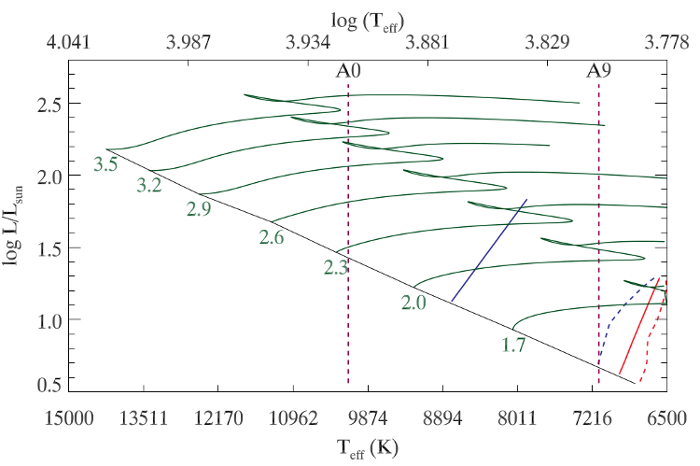
\includegraphics[width=\linewidth]{Chapter3/Astar_evol_tracks.png}
    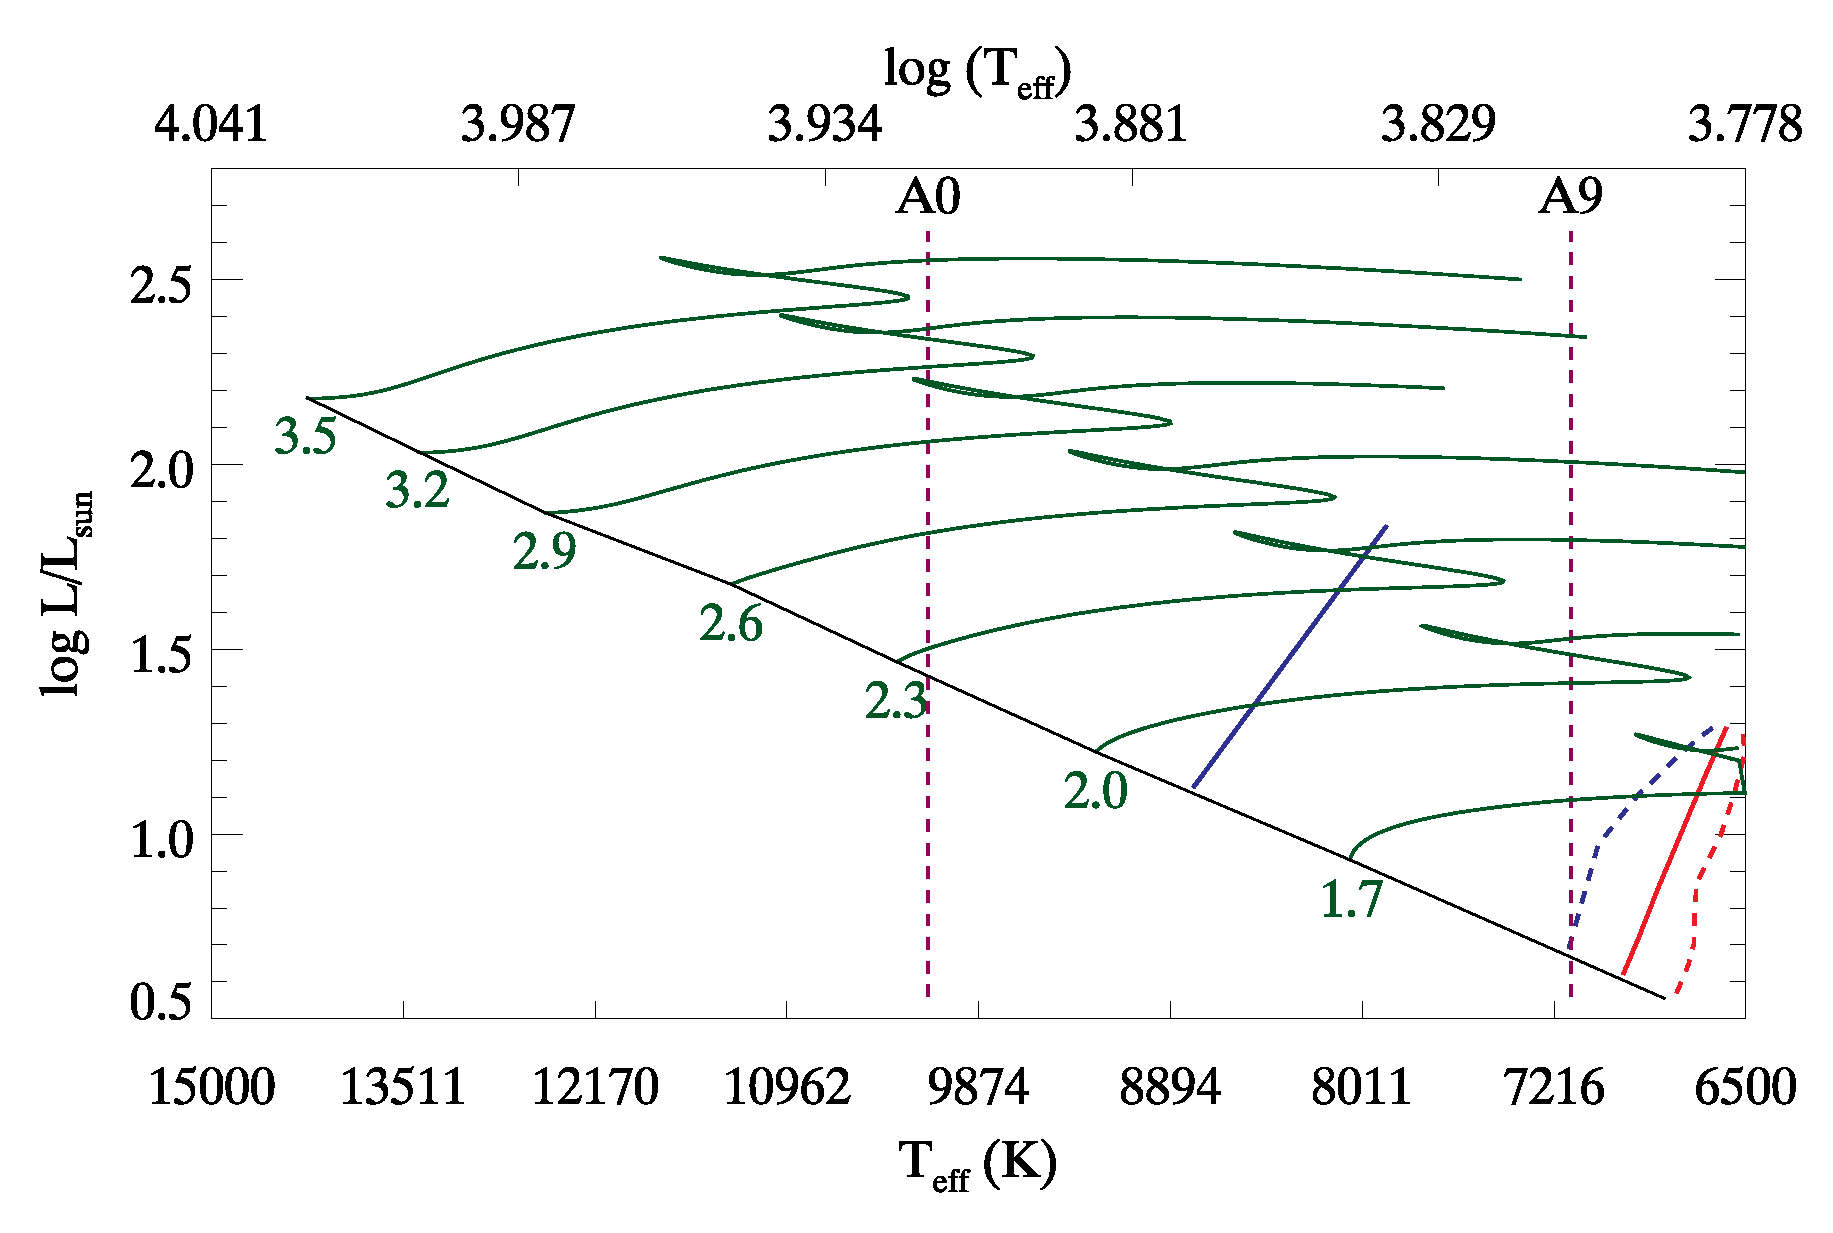
\includegraphics[width=\linewidth]{Chapter3/A_star_HR_delimited.eps}
    \caption[HR diagram with evolutionary tracks of A-type stars]{HR diagram between early-B and late-F spectral regions, reproduced from \citet{murphy_examination_2012}. Evolutionary tracks for 1.7\,\Msol~to 3.5\,\Msol~stars are plotted in green and corresponding masses given below the ZAMS (black). The A-type star boundaries are delineated with dashed purple lines at 10\,150\,K (A0) and 7\,150\,K (A9).}
    \label{fig:Astar_evol_tracks}
\end{figure}

% HR diagram covering the late-B to early-F region (spectral types A0
% and A9 are delimited). A star at A0 has a surface temperature of ∼10 150 K, and
% at A9 ∼7150 K. Evolutionary tracks are plotted in green, with their corresponding
% masses (in M ) written just below the zero-age main sequence (black). The principal
% direction of evolution for the B stars is to the right, such that they become A stars.
% For reference, the δ Sct instability strip’s red and blue edges are plotted as solid lines,
% and the γ Dor strip as dashed lines. Tracks were calculated using time-dependent
% convection (TDC) models, and contributed by A. Grigahcène (priv. comm.).

%As a class, the chemically peculiar A type (Ap) stars exhibit enhanced features of rare earth elements, such as Sr, Cr and Eu, in their spectra \citep{Morgan1933Evidence}. This enhancement is the result of a stable magnetic field on the order of a few to tens of kG \citep{Mathys2017Ap}, which typically allows for the formation of abundance `spots' on the surface, concentrated at the magnetic poles \citep{Ryabchikova2007Pulsation}. In most, but not all Ap stars, photometric and spectral variability over the rotation cycle can be observed \citep{Stepien2000Loss, Abt1995Relation}. Such characteristic spot-based modulation manifests as a low frequency modulation of the light curve which is readily identified, allowing for the rotation period to be measured \citep[e.g.][]{Drury2017Large}.
%As such, they are greatly outnumbered by the much more abundant non-oscillating Ap stars \citep{Renson2009Catalogue,Ghazaryan2018New}.

% Since their discovery by \citet{Kurtz1982Rapidly}, only 61 rapidly oscillating Ap (roAp) stars have been found. Understanding of their pulsation mechanism, occurrence rate, and origin of magnetic fields have all been hindered by the relatively small number of known roAp stars. A key difficulty in their detection lies in the rapid oscillations themselves, requiring dedicated observations from ground or space-based photometry at a short enough cadence to properly sample the oscillations. In this paper, we show that the \kepler\ long-cadence data can be used to detect roAp stars.

% The roAp stars are a rare subclass of the chemically peculiar A-type stars, which exhibit rapid brightness and radial velocity variations with periods between 5 and 25 min and amplitudes up to 0.018 mag in Johnson $B$ \citep{Kurtz2000Introduction, Kochukhov2009Asteroseismology, Smalley2015KIC}. They oscillate in high-overtone, low-degree pressure (p) modes \citep{Saio2005Nonadiabatic}. The excitation of high overtone p-modes, as opposed to the low overtones of other classical instability strip pulsators, is suspected to be a consequence of the strong magnetic field -- on the order of a few to tens of kG -- which suppresses the convective envelope at the magnetic poles and increases the efficiency of the opacity mechanism in the region of hydrogen ionisation \citep{Balmforth2001Excitation,Cunha2002Theoretical}. Based on this, a theoretical instability strip for the roAp stars has been published by \citet{Cunha2002Theoretical}. However, discrepancies between the observed and theoretical red and blue edges have been noted, with several roAp stars identified to be cooler than the theoretical red edge. 

% A further challenge to theoretical models of pulsations in magnetic stars is the existence of stars which oscillate above the so-called acoustic cutoff frequency \citep{Saio2013Pulsation,Holdsworth2018LCO}. In non-magnetic stars, oscillations above this frequency are not expected. However, in roAp stars the strong magnetic field guarantees that part of the wave energy is kept inside the star in every pulsation cycle, for arbitrarily large frequencies \citep{sousaandcunha2008}. For that reason, no theoretical limit exists to the frequency of the modes. Nevertheless, for a mode to be observed, it has to be excited. Models show that the opacity mechanism is capable of exciting modes of frequency close to, but below, the acoustic cutoff frequency. The excitation mechanism behind the oscillations with frequencies above the acoustic cutoff is thought to be turbulent pressure in the envelope regions where convection is no longer suppressed \citep{Cunha2013Testing}.

% The magnetic field axis of roAp stars is closely aligned with the pulsation axis, with both being inclined to the rotation axis. Observation of this phenomenon led to the development \citep{Kurtz1982Rapidly} and later refinement \citep{Dziembowski1985Frequency,Shibahashi1985Rapid,Shibahashi1985Rotational,Shibahashi1993Theory,Takata1994Selection,Takata1995Effects,Bigot2011Theoretical} of the oblique pulsator model. The roAp stars present a unique testbed for models of magneto-acoustic interactions in stars, and have been widely sought with both ground and space-based photometry.

\subsection*{Declaration}
The work presented in this publication was begun during my Honours year and completed in the course of this PhD. I extracted and processed the light curve using my own custom-defined aperture from superstamps that I stitched together. I conducted the Fourier analysis of the light curve searching for oscillation signatures and determined none were detectable above the signal-to-noise threshold. The multi-colour photometry was obtained by Aliz Derekas et. al. who eliminated the possibility of classification as a Cepheid for this star. The Nordic Optical Telescope (NOT) observations were conducted as part of the NOT `Fast-track' service time. Simon Murphy identified the chemically peculiar signatures of Europium, Strontium and Chromium as well as annotating the stellar spectrum. \'Ad\'am S\'odor conducted the model-based rotational modulation stability analysis that improved upon my initial polynomial-based O-C results. The analysis and writing of this paper was conducted by me in conjunction with my supervisors Dennis Stello and Tim Bedding.

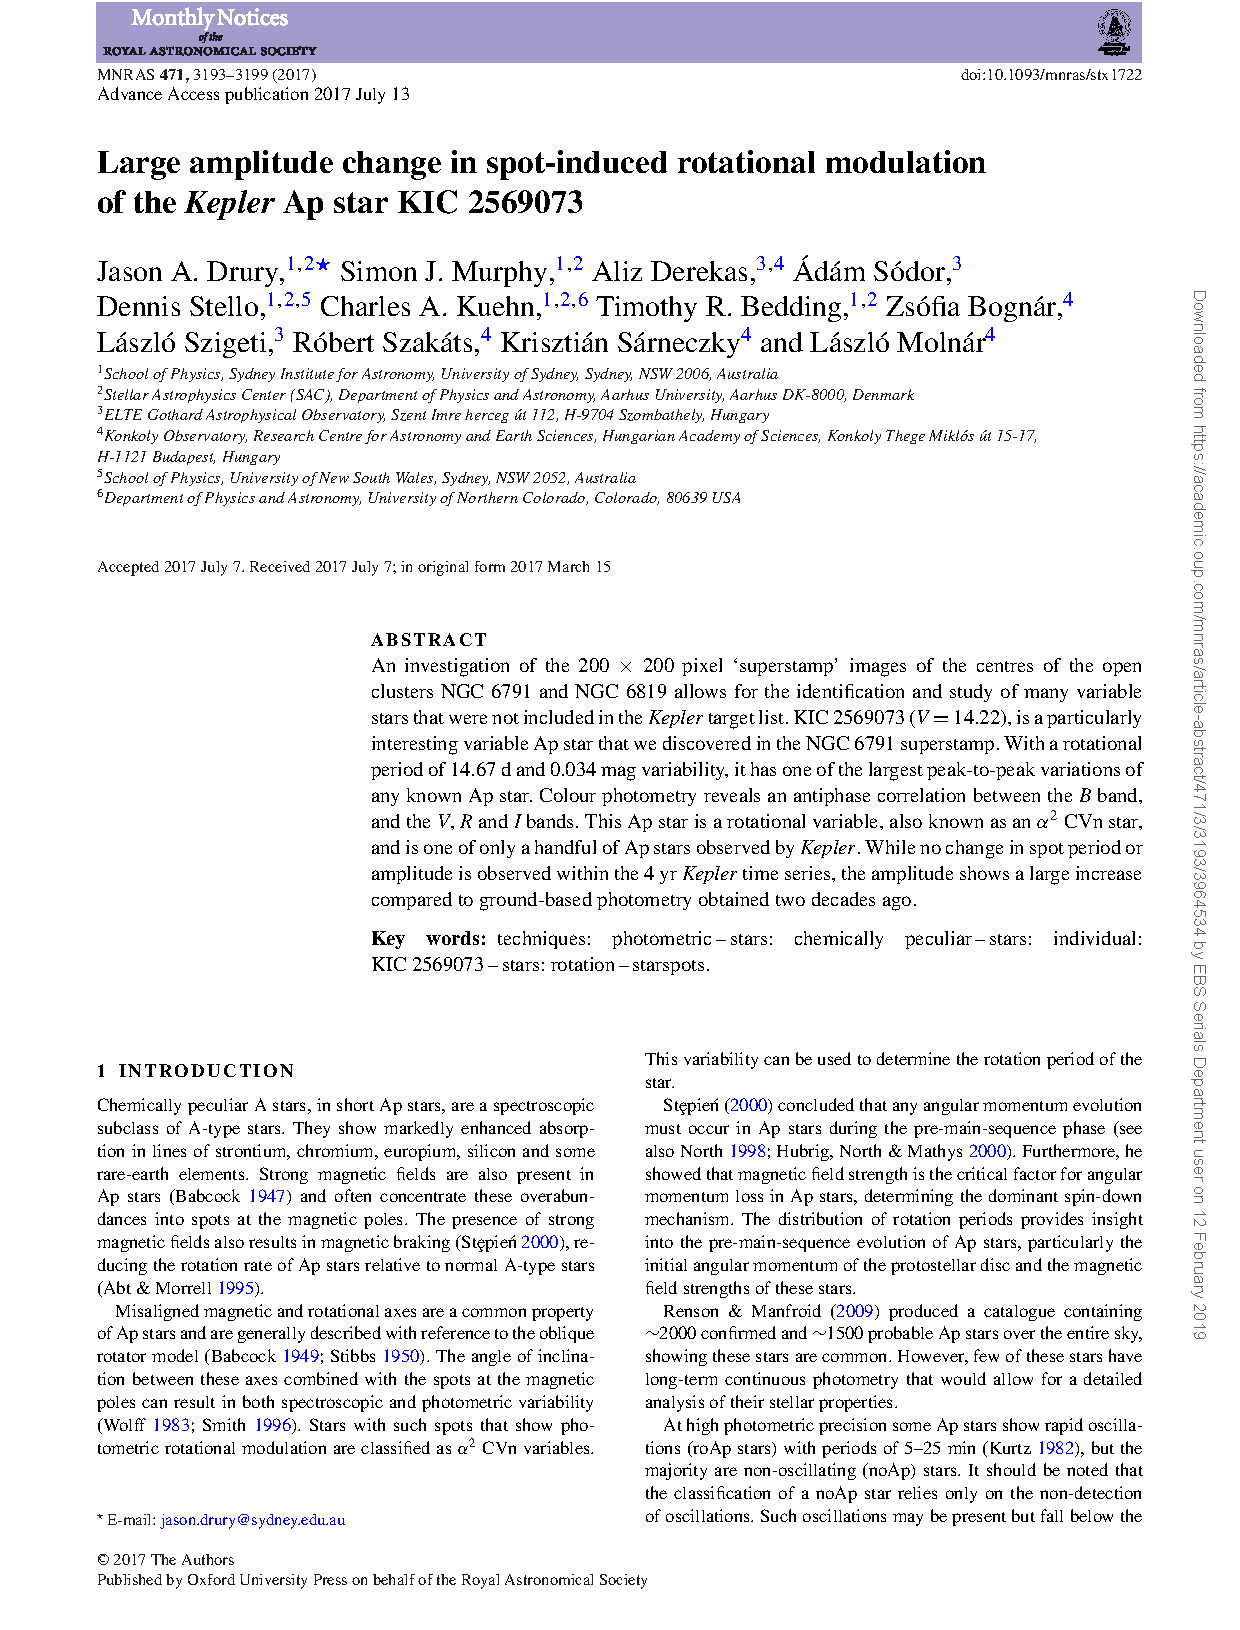
\includepdf[pages=-,pagecommand={},width=1.1\linewidth]{Papers_PDF/KIC2569073.pdf}